\documentclass{beamer}
\usetheme{Warsaw} % Madrid Antibes Warsaw
\setbeamertemplate{navigation symbols}{}
% \setbeamertemplate{}{}
\usepackage[utf8]{inputenc}
\usepackage[english]{babel}
\usepackage{pgfplots}
% \usepackage{amssymb}
% \usepackage{amsmath}
% \usepackage{mathrsfs}
% \usepackage{microtype}


\title[Ph.D. Completion Seminar]{A Big Data Infrastructure for Real-time Traffic Analytics on the Cloud}
\subtitle[]{Ph.D. Completion Seminar}
\institute[Unimelb]{\sc The University of Melbourne \vspace{5pt} \\ Australia }
\author[Yikai Gong \hspace{0.1\textwidth} \insertframenumber\,/\,\inserttotalframenumber]{ Yikai Gong \\ \texttt{yikaig@student.unimelb.edu.au}
\\ \vspace{10pt} \small{Supervisor: Prof. Richard O. Sinnott \\Co-Supervisor: Prof. Stephan Winter}
}
\date{April 15, 2019}

\begin{document}
\begin{frame}[plain]
    \maketitle
\end{frame}

\begin{frame}[plain]
    \frametitle{Table of Contents}
    \tableofcontents[]
\end{frame}

%==============================
\section{Introductions}
%==============================

%----------------------------
\subsection{Motivations}

\begin{frame}
    \frametitle{Why (Real-time) Urban Traffic Analytics is Important?}
    \begin{itemize}
	    \item The Urban Traffic Issue is a common and critical challenge facing all modern cities. Traffic congestions have many impacts other than simply causing delays, e.g, pollution, health, livability, et al.
	    \item Traffic can cost huge amounts of money to address --- typically at the taxpayers expense.
	    \begin{itemize}
            \item The government of Victoria in Australia made a 10-year, ${\$75}$ billion budget available for transport infrastructure in 2018~\cite{10YInvVic}.
            \item This raises many questions to the city planners regarding urban infrastructure and especially in understanding the status of daily traffic and steps that may be taken to reduce traffic congestion.
        \end{itemize}
        \item The status of urban traffic is time-sensitive. Real-time traffic analysis/service can help individual to avoid traffic issues, e.g, Google Traffic Service.
    \end{itemize}
\end{frame}

\begin{frame}
    \frametitle{Using Big Data for Analyzing Urban Traffic}
    \begin{itemize}
	    \item A large volume of digital data is being created across all walks of life by industry, governments and society, e.g., sensor network, Internet of Things (IoT), Social Media, Official records et al.
	    \item The emergence of ''Big Data'' raise many new opportunities and challenges for analyzing the Urban Traffic.
	    \begin{itemize}
	        \item Can we build a generic platform that meet all the requirements for real-time Urban Traffic Analytics using Big Data?
	    \end{itemize}
	    \item The accurate official Urban Traffic data are expensive to collect due to the installation and maintenance of the specialized devices, e.g., sensor network. 
	    \begin{itemize}
	        \item Is it possible to find a ''cheaper'' proxy for Urban Traffic?
	    \end{itemize}
    \end{itemize}
\end{frame}


%----------------------------
\subsection{Related Works}

\begin{frame}
    \frametitle{Tackling the Big Data Challenges}
    \begin{itemize}
	    \item There are existing solutions, i.e, Cloud Computing, to deal with many of the common Big Data challenges regarding to:
	        \begin{itemize}
	            \item High Volume
	            \item High Velocity
	            \item High Variety
	        \end{itemize}
	    \item In addition to the common Big Data challenges, Urban Traffic data and its related analysis have unique characteristics that need to be addressed:
	    \begin{itemize}
	        \item Storing and indexing geographic (traffic) Big Data.
	        \item Geographic (complex) processing on Big Data.
	        \item Visualization of Traffic Big Data and its analyzed results.
	    \end{itemize}
    \end{itemize}
\end{frame}

\begin{frame}
    \frametitle{Urban Traffic Analytics}
    \begin{itemize}
	    \item The typical class of methods for traffic analysis is modeling traffic data for subsequent traffic flow detection and forecasting.
	    \begin{itemize}
	        \item The building of these models can involve complex calculations, e.g, vector-based regression models~\cite{cao2007robust}, artificial neural network models~\cite{ye2009neural}, et al.
	        \item The speed of processing is often a key requirement for traffic forecasting.
	    \end{itemize}
	    \item Social media data has become a popular data source for a range of Urban research scenarios including traffic analysis \cite{feldman2013techniques}.
	    \begin{itemize}
	        \item Many of these works focus on the contents of social media data, i.e, Natual Language Processing (NPL) based methods.
	        \item The spatio-temporal feature of social media data could provide more reliable information for urban traffic analysis.
	    \end{itemize}
    \end{itemize}
\end{frame}

%----------------------------
\subsection{Research Hypthesis}

\begin{frame}
    \frametitle{Research Hypthesis}
    It is possible to develop a big data processing platform for urban transport that targets the specific needs, demands and challenges of big data including the volume, velocity, and variety of urban traffic data.

    \begin{block}{Sub-hypotheses 1}
    Is it possible to use social media data as a proxy for official traffic data that is more expensive and difficult to collect?
    \end{block}
    \begin{block}{Sub-hypotheses 2}
    Are there new spatio-temporal algorithms that need to be realised to address the specific challenges around the analysis of real-time traffic/social-media data?
    \end{block}
\end{frame}

%==============================
\section{Methodologies}
%==============================

%----------------------------
\subsection{Utilizing the Geo-information of Social Media}
\begin{frame}
    \frametitle{Idea and Data Resource}
    \begin{itemize}
	    \item Idea:
	    \begin{itemize}
	        \item Utilizing the geo-tags in social media data.
	        \item Can we use the spatio-temporal clusters of social-media data on/near the road-network for identifying traffic issues, e.g, congestions?
	    \end{itemize}
	    \item Data Resource:
	    \begin{itemize}
	        \item Social Media data: Tweets collected from the Twitter public API.
	        \item Road network data: PSMA Road data
	    \end{itemize}
    \end{itemize}
\end{frame}

\begin{frame}
    \frametitle{Harvesting Twitter data along streets using PSMA}

    \begin{figure}[h]
       \begin{minipage}{0.49\textwidth}
         \centering
         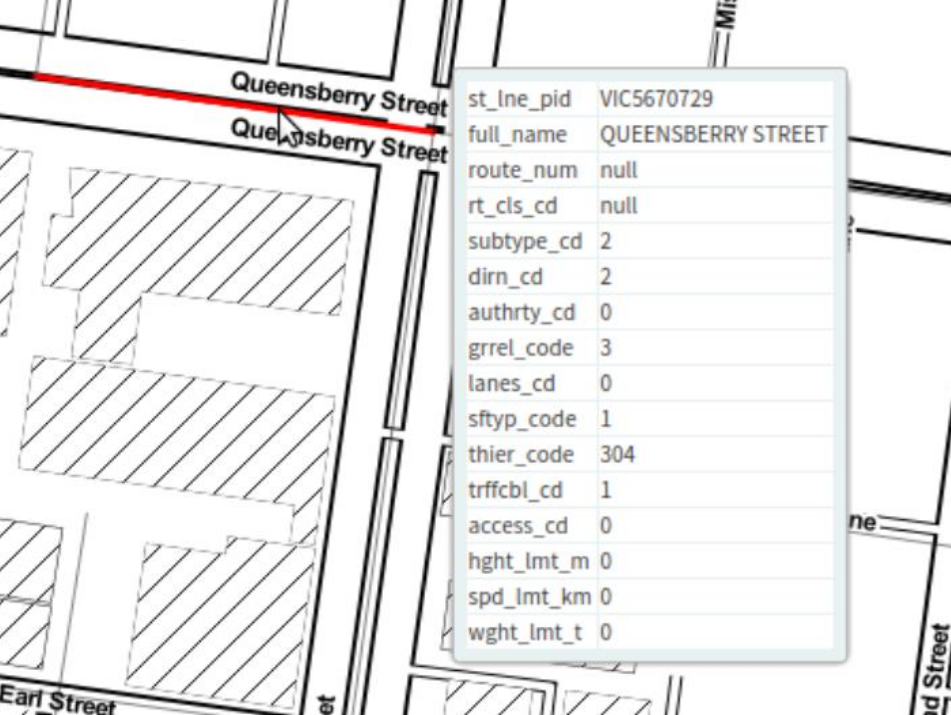
\includegraphics[width=.8\linewidth]{resource/figures/psma_data.png}
         \caption{An example of PSMA road data}\label{fig:psma}
       \end{minipage}\hfill
       \begin{minipage}{0.49\textwidth}
         \centering
         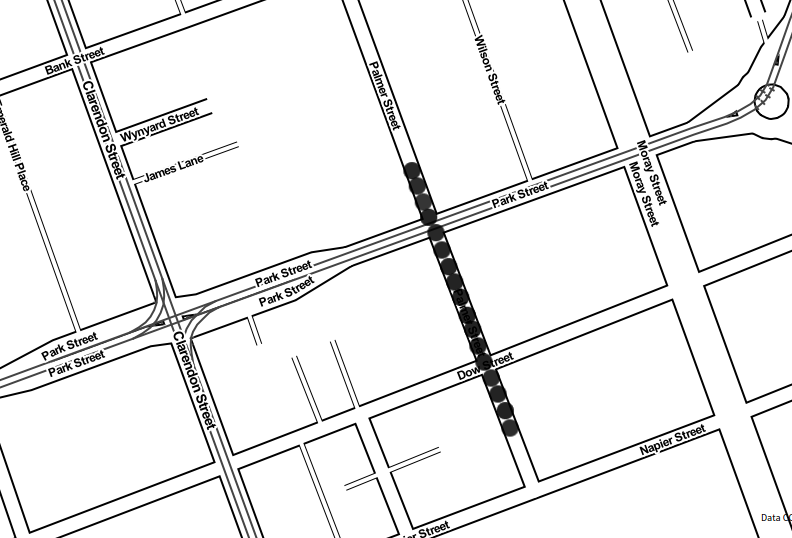
\includegraphics[width=.8\linewidth]{resource/figures/harvest_tweets_along_street.png}
         \caption{A serial of bounding boxes for harvesting tweets along streets}\label{fig:harvest_along_street}
       \end{minipage}
    \end{figure}

    \begin{itemize}
	    \item Generate queries (bounding box) based on the PSMA data and collect data along streets
    \end{itemize}
\end{frame}

\begin{frame}
    \frametitle{Clustering the Social Media Data using DBSCAN}
    \begin{columns}
          \column{0.35\linewidth}
             \centering
             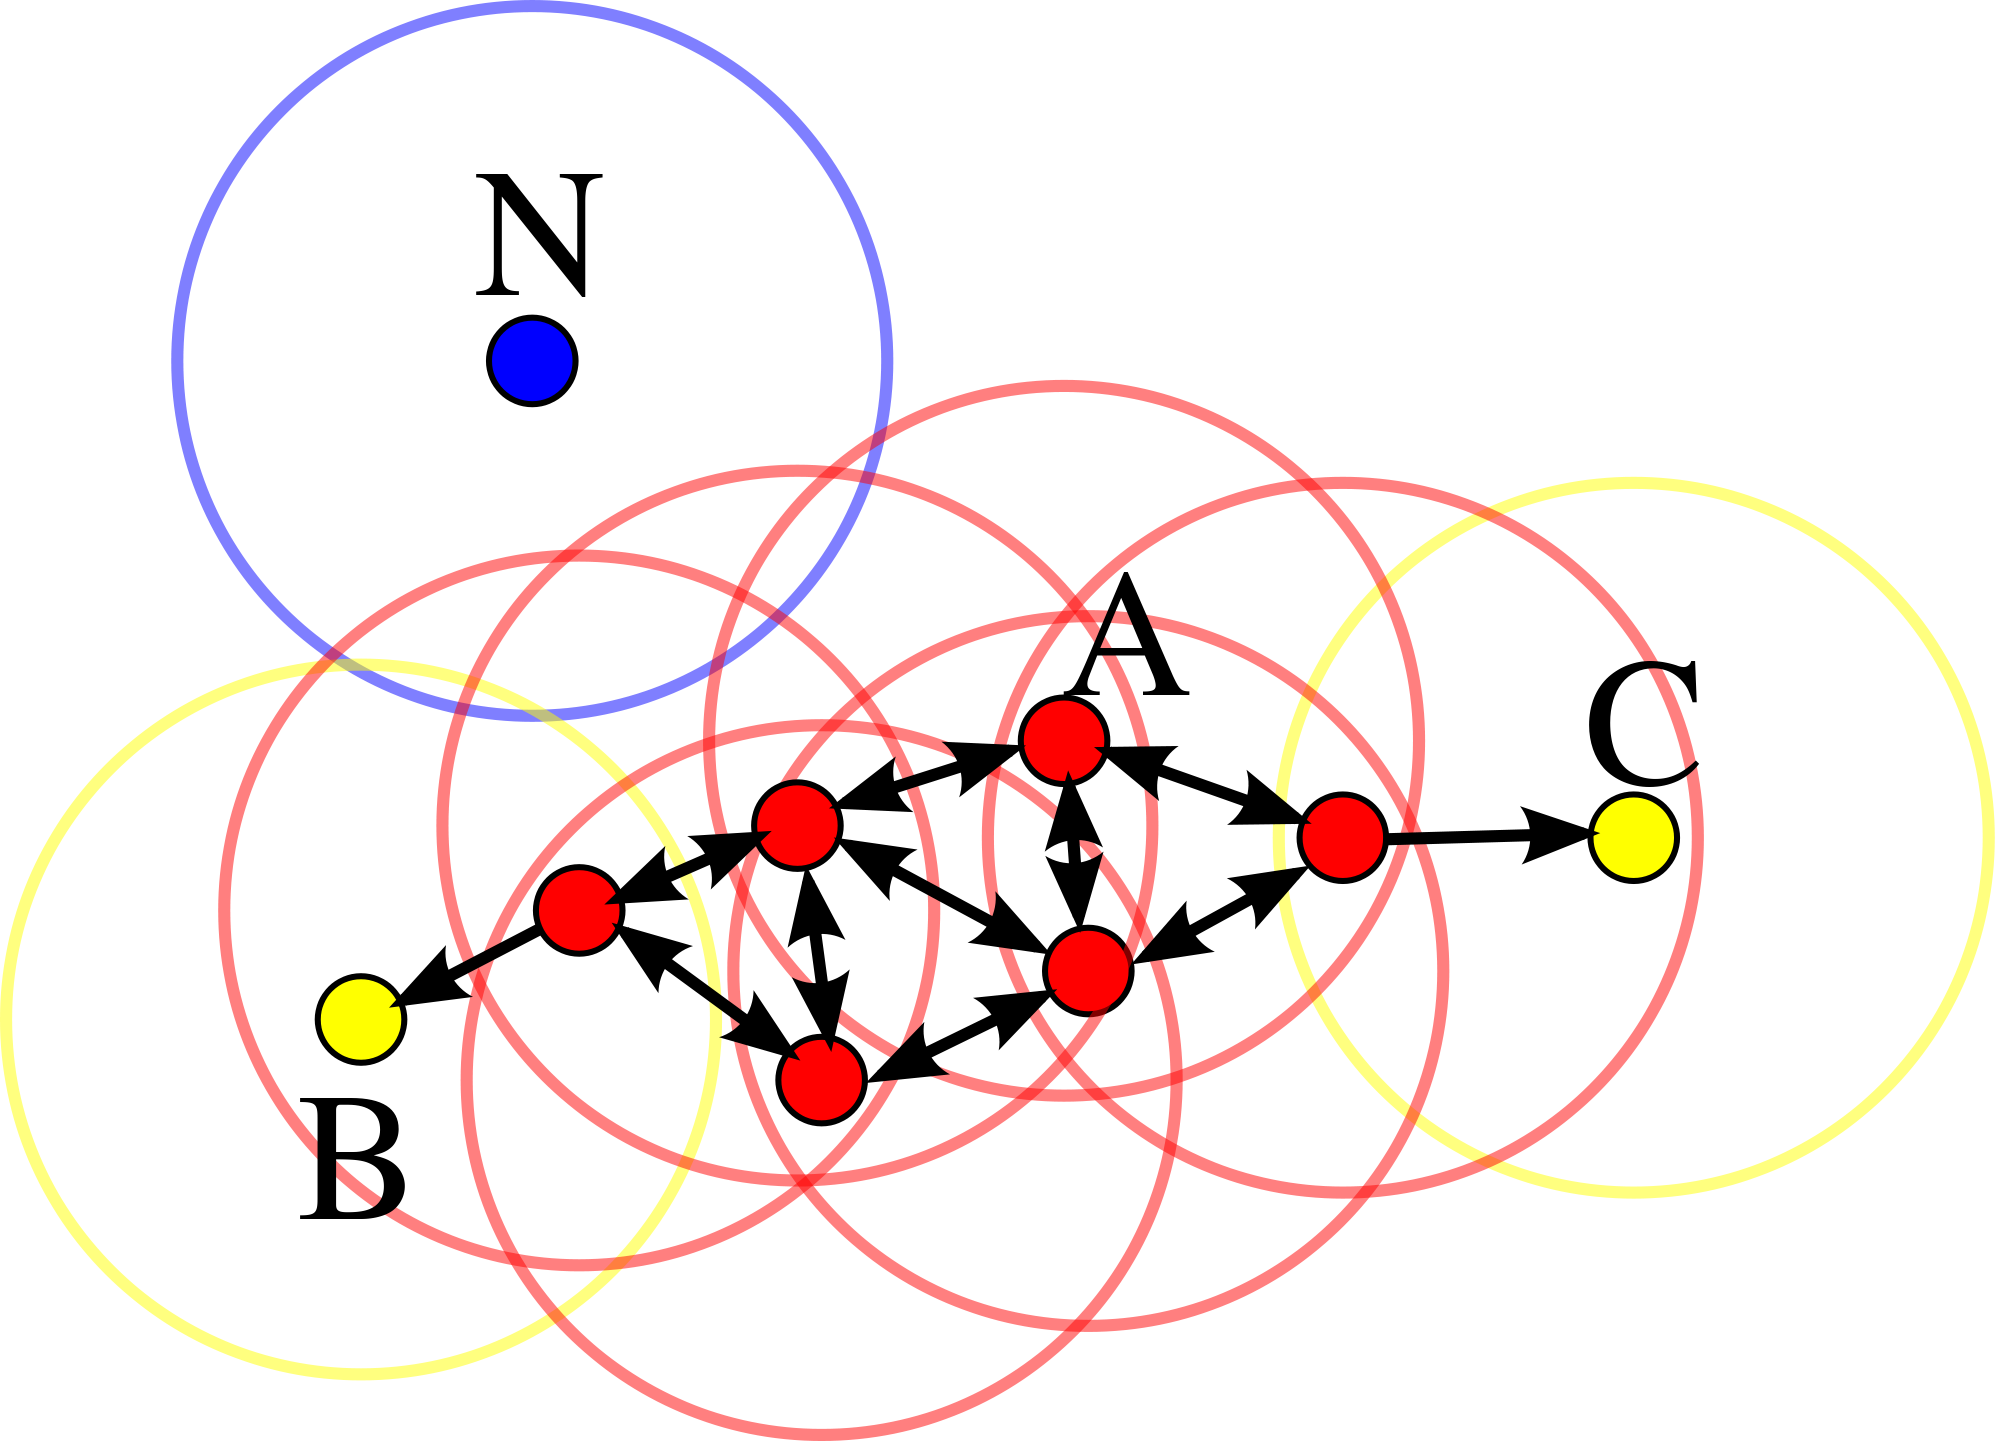
\includegraphics[width=\textwidth]{resource/figures/dbscan.png}\\
              \tiny \textit{Given a set of points in some space, it groups together points that are closely packed together, marking as outliers points that lie alone in low-density regions.}
           \column{0.65\linewidth}
              \begin{itemize}
                  \item To identify clusters of tweets in space and time.
                  \item Based on DBSCAN algorithm
                  \begin{itemize}
                      \item Parameters for identification:
                      \begin{itemize}
                          \item Distance - $\epsilon$
                          \item Minimum number of points - $minPts$
                      \end{itemize}
                      \item A cluster is formed when a set of data points are close to each other with the total number of points no less than $minPts$.
                  \end{itemize}
              \end{itemize}
              \begin{block}{Spatio-temporal Distance (STD)}
                $STD = \frac{TimeDistance}{2} + \frac{SpatialDistance}{2}$
              \end{block}
    \end{columns} 
\end{frame}

\begin{frame}
    \frametitle{Results and Architecture}
    \begin{figure}[h]
       \begin{minipage}{0.5\linewidth}
         \centering
         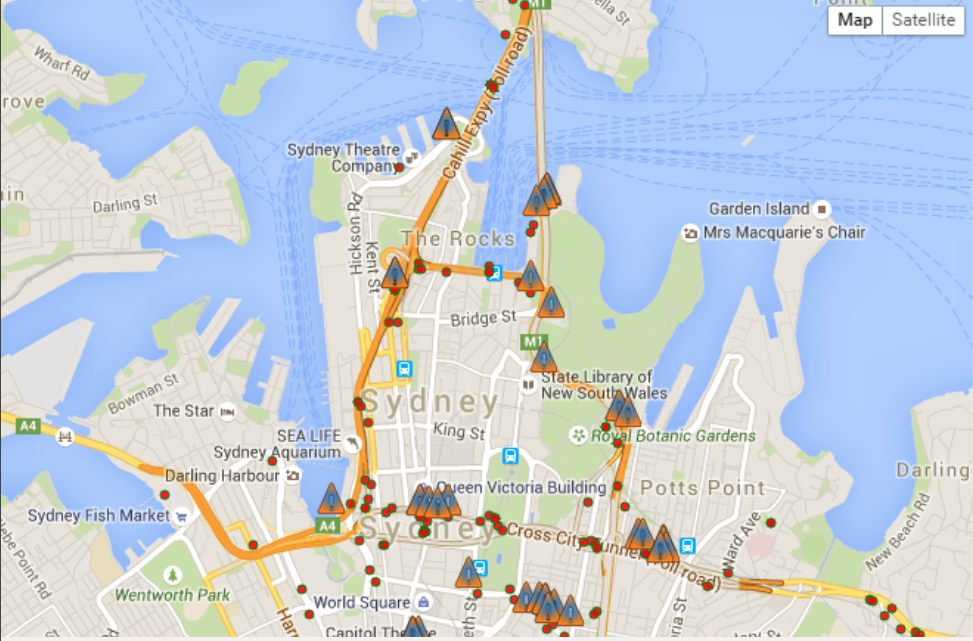
\includegraphics[width=.8\linewidth]{resource/figures/harvester_cluster_3.png}
         \caption{Detected tweets clusters (triangles) and noise data (red points) in Sydney on 07/05/2015}
       \end{minipage}\hfill
       \begin{minipage}{0.5\linewidth}
         \centering
         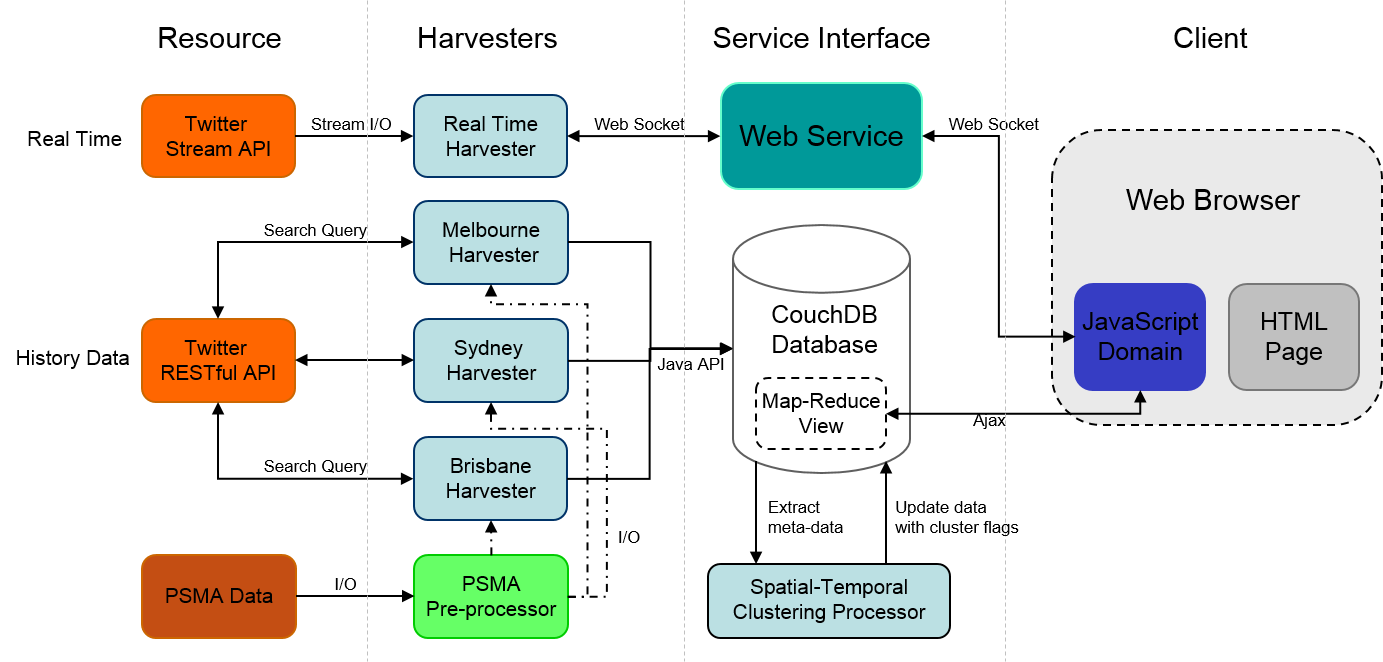
\includegraphics[width=.8\linewidth]{resource/figures/harvester_architecture.png}
         \caption{Software Architecture for Harvesting and Clustering Tweets}
       \end{minipage}
    \end{figure}
    \vspace{-0.3cm}
    \begin{itemize}
        \item Need to explore the correlation between social media clusters and traffic data/status
        \item Need a cloud-based platform to conduct the case-studies for analyzing (real-time) urban traffic issues.
    \end{itemize}
\end{frame}

%----------------------------
\subsection{The SMASH architecture for Urban Traffic Analytics}
\begin{frame}
    \frametitle{Architecture Requirements}
    \begin{itemize}
	    \item Continual growth of large volumes of data.
	    \item Multiple heterogeneous data stream coming at a high velocity.
	    \item Ability to index and query large-scale geospatial data.
	    \item Ability to apply existing/general processing methods related to urban traffic.
	    \item Processing Big Data stream in (near) real-time. 
	    \item Visualization of data and results of urban traffic analytics.
    \end{itemize}
\end{frame}

\begin{frame}
    \frametitle{The SMASH architecture}
    \begin{columns}
          \column{0.35\linewidth}
             \begin{figure}
                 \centering
                 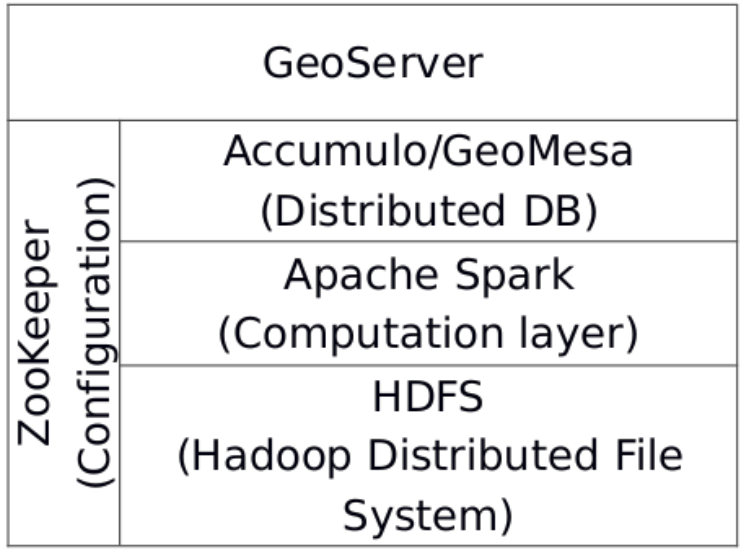
\includegraphics[width=\textwidth]{resource/figures/smash_architecture.png}
                 \caption{Software stack of SMASH}
             \end{figure}
           \column{0.65\linewidth}
              \begin{itemize}
                \item A scalable architecture based on IaaP Cloud Infrastructure.
                \item A software stack running in a computing cluster.
                \item Dockerized deployment make it flexible to be scaled and deployed across multiple Clouds, i.e, Hybrid Cloud.
              \end{itemize}
    \end{columns}
\end{frame}

%----------------------------
\subsection{Dockerized Deployment of SMASH and Benchmark}
\begin{frame}
    \frametitle{Dockerized Deployment of SMASH}
    \begin{figure}
        \centering
        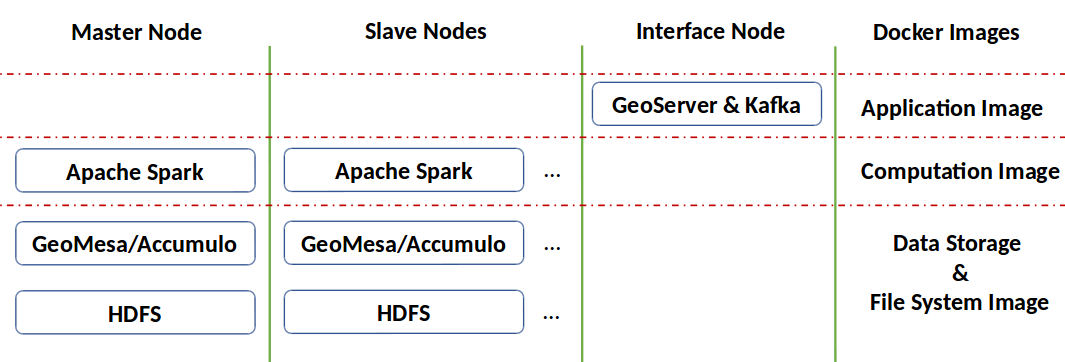
\includegraphics[width=\linewidth]{resource/figures/smash-docker.png}
        \caption{High-level SMASH Software Architecture and its Dockerized Implementation}
    \end{figure}
\end{frame}

\begin{frame}
    \frametitle{Benchmarking SMASH}
    \begin{columns}
          \column{0.5\linewidth}
             \vspace{-0.5cm}
             \begin{figure}
                 \centering
                 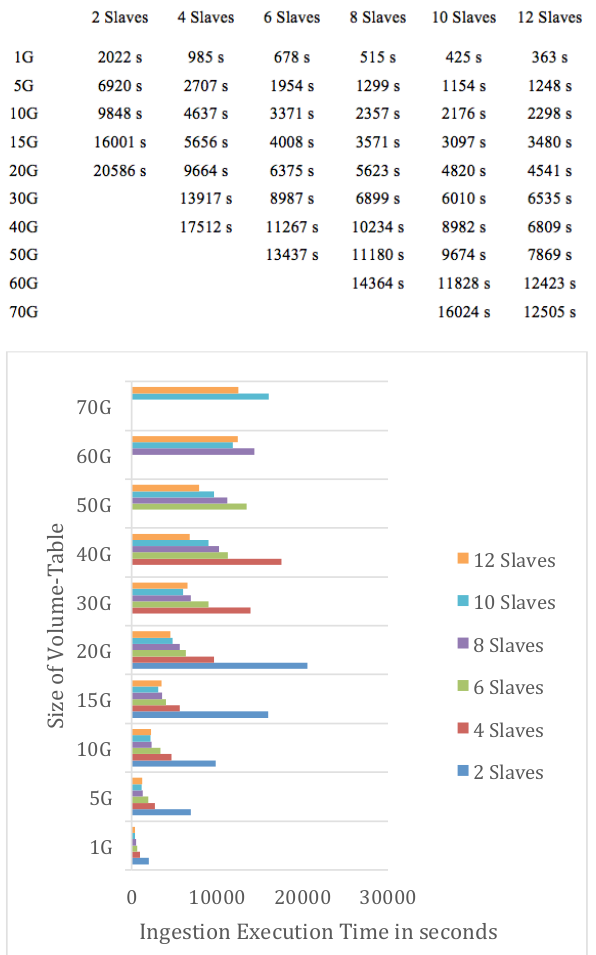
\includegraphics[height=6cm]{resource/figures/benchmark_ingest.png}
                 \vspace{-0.4cm}
                 \caption{\tiny Benchmarking Data Ingestion}
             \end{figure}
           \column{0.5\linewidth}
             \vspace{-0.5cm}
             \begin{figure}
                 \centering
                 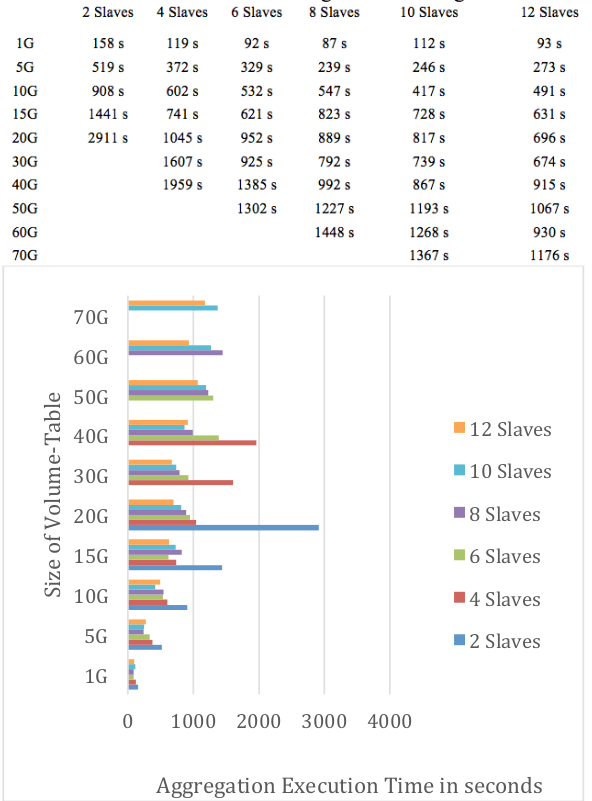
\includegraphics[height=6cm]{resource/figures/benchmark_aggregate.png}
                 \vspace{-0.4cm}
                 \caption{\tiny Benchmarking Data Aggregation}
             \end{figure}
    \end{columns}
\end{frame}

%----------------------------
\subsection{Real-time Density-based Clustering Algorithm (RT-DBSCAN)}

\begin{frame}
    \frametitle{The Requirements of Real-time Clustering Algorithm}
    \begin{itemize} \small
	    \item There is a strong need for real-time cluster discovery in many time-sensitive domains such as:
        \begin{itemize} \small
            \item Urban traffic monitoring.
            \item Emergency response.
            \item Network accessing analysis
        \end{itemize}
	    \item The demands for real-time clustering of big data raise several requirements, including:
        \begin{itemize} \small
            \item Generate a series of up-to-date intermediate result check-points when processing real-time (incoming) data stream.
            \item Support scalable parallel execution capabilities to reduce the response time for generating checkpoints. 
            \item Offer consistent performance in tackling ever growing amounts of data.
        \end{itemize}
        \begin{figure}
            \centering
            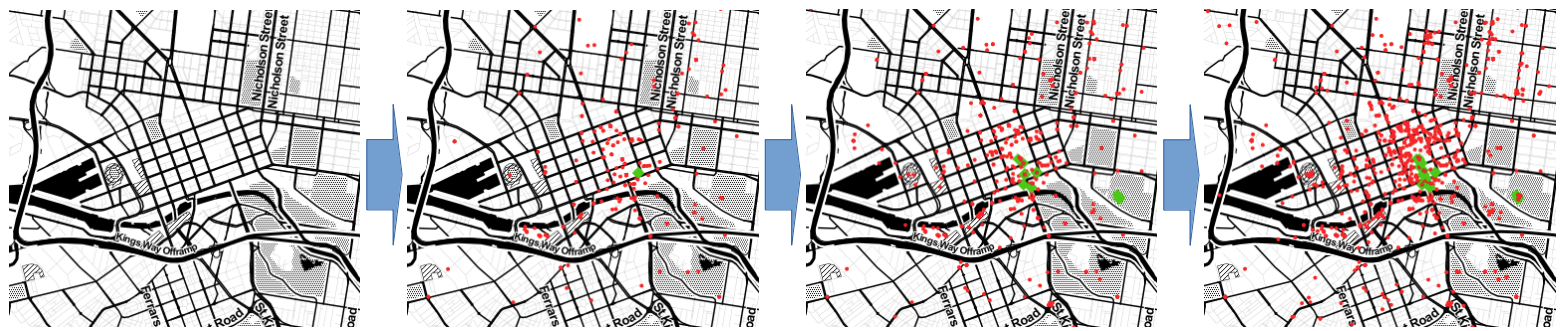
\includegraphics[width=0.6\linewidth]{resource/figures/cluster_checkpoints.png}
        \end{figure}
    \end{itemize}
\end{frame}

\begin{frame}
    \frametitle{A Review of Traditional DBSCAN}
    \begin{columns}
          \column{0.4\linewidth}
             \centering
             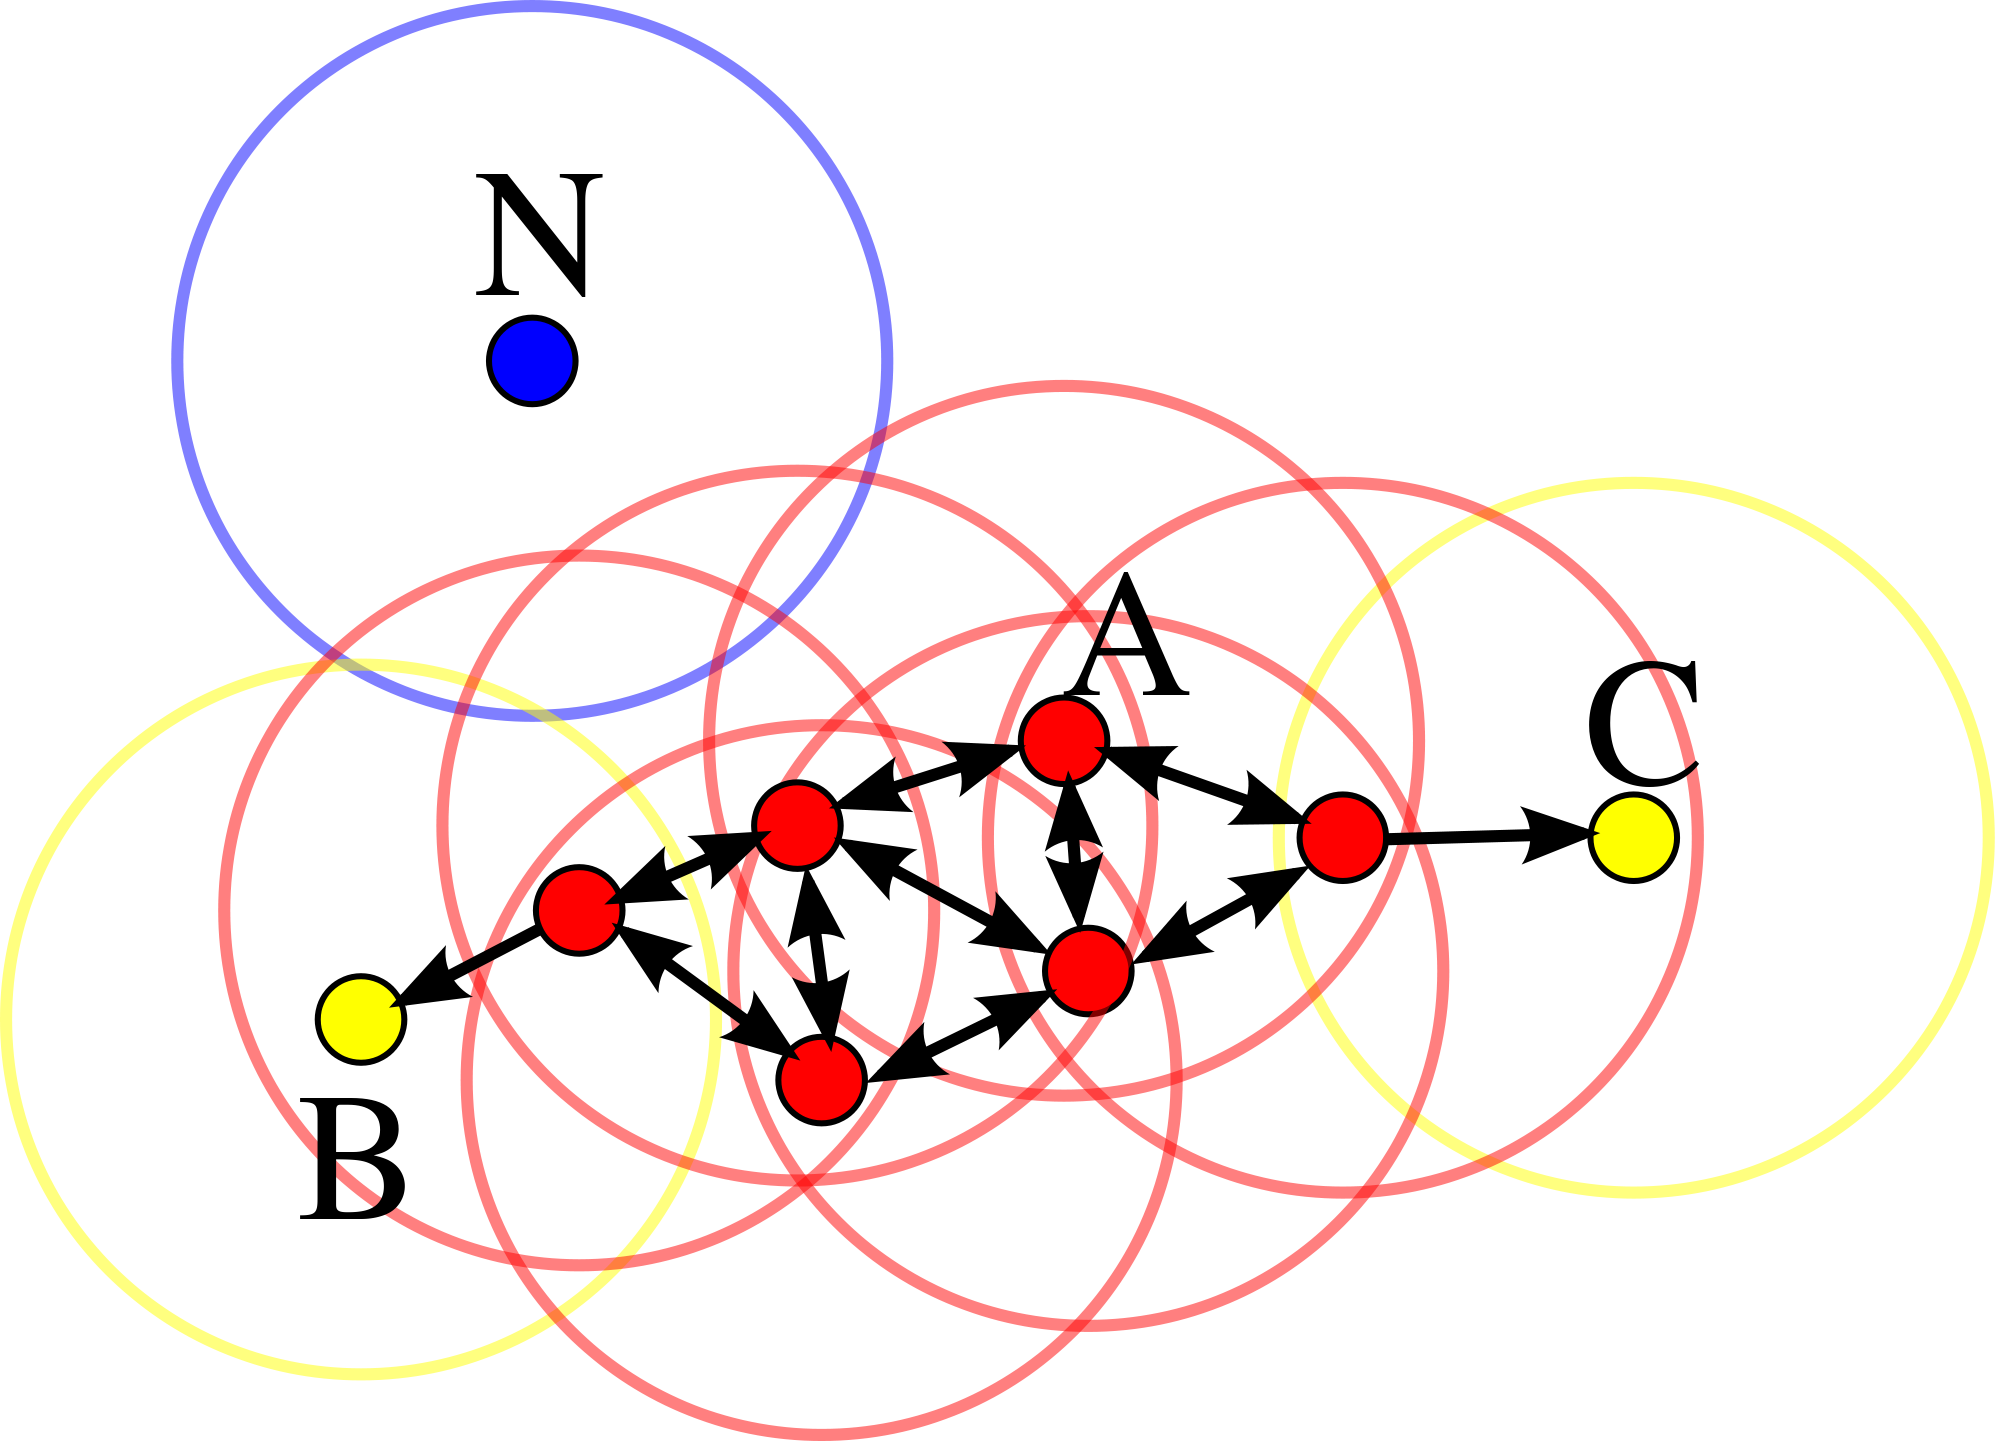
\includegraphics[width=\textwidth]{resource/figures/dbscan.png}
           \column{0.6\linewidth}
              \begin{itemize}
                  \item Density-based spatial clustering of applications with noise.
                  \begin{itemize}
                      \item Preset Parameters:
                      \begin{itemize}
                          \item Distance - $\epsilon$
                          \item Minimum number of points - $minPts$
                      \end{itemize}
                  \end{itemize}
              \end{itemize}
    \end{columns} 
    \vspace{0.3cm}
    \begin{itemize}
        \item DBSCAN is one of the most common clustering algorithms and also most cited in scientific literature.
        \begin{itemize}
            \item Not require to set the number of clusters in prior.
            \item Ability to identify arbitrary shaped clusters and outliers.
            \item Customized distance measurement – For non spatial data.
        \end{itemize}
    \end{itemize}
\end{frame}

\begin{frame}
    \frametitle{Challenges and Solutions of real-time DBSCAN clustering }
	    Main challenge of real-time DBSCAN clustering:
        \begin{itemize}
            \item Controlling the size of traversal data needed to cluster ever growing data volumes
            \begin{itemize}
                \item  Complexity of the classic DBSCAN $~$ $O(n^2)$
                \item  Typical DBSCANs traverse the whole dataset, and identifies the neighbors of each point. Each data element can be processed multiple times
            \end{itemize}
        \end{itemize}
	    The idea of our solution:
	    \begin{itemize}
	        \item \small For each new input point, if there is an efficient way to identify a full set of essential near-by points in the historical dataset, only this subset of data is needed for clustering against any new input.
            \item \small If the performance of this pre-filtering method is not sensitive to the size of dataset, then we can cluster real-time stream data on-the-fly without being challenged by the ever growing volume of data.
	    \end{itemize}
\end{frame}

\begin{frame}
    \frametitle{Find the essential nearby knowledge for each input}
    \begin{columns}
          \column{0.7\textwidth}
             \centering
             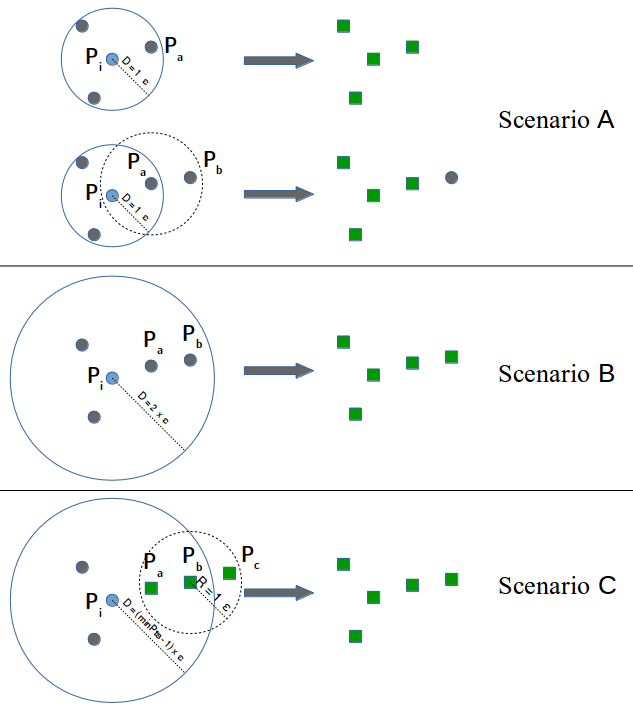
\includegraphics[width=0.8\textwidth]{resource/figures/context.png}
           \column{0.55\textwidth}
            DBSCAN parameters:
            \begin{itemize}
                \item $\epsilon = 1 unit$
                \item $minPts = 3$
            \end{itemize}
            \vspace{1cm}
            Radius (minDis) for getting \\essential nearby knowledge
            \begin{itemize}
                \item \small $minDis = (minPts - 1) \times \epsilon$
            \end{itemize}
    \end{columns}
\end{frame}

\begin{frame}
    \frametitle{Point-by-point Growing of DBSCAN clusters}
    Insert input Data into Existing Cluster Patterns one by one.
    \begin{itemize}
	    \item Build connections between input points and nearby points.
	    \item Build rules for all the possible conditions:
    \end{itemize}
    \begin{columns}
          \column{0.5\textwidth}
            \centering
            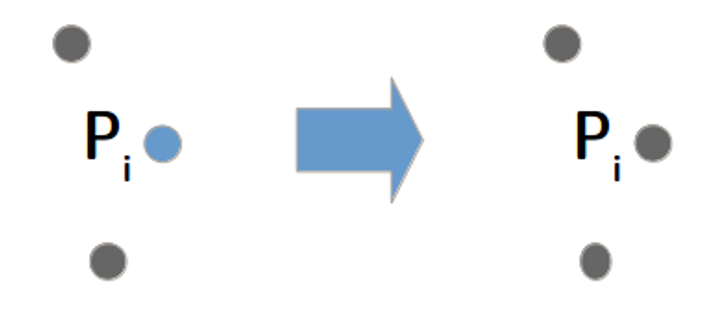
\includegraphics[width=0.8\textwidth]{resource/figures/condition1.png}
            \\ \tiny New noise data.
           \column{0.5\textwidth}
            \centering
            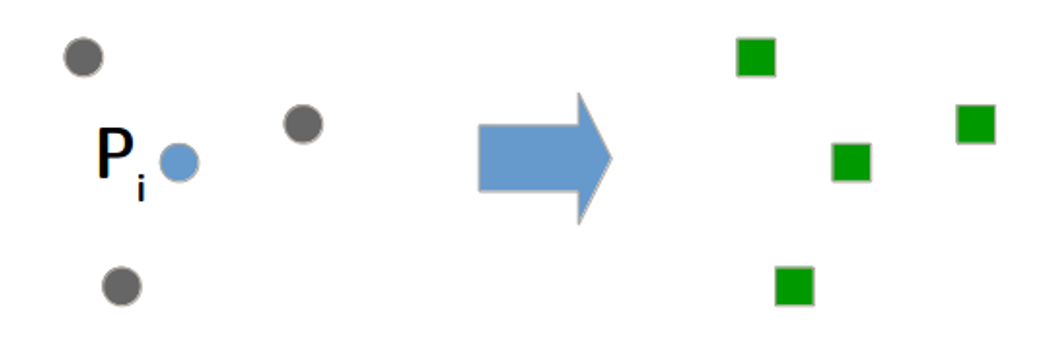
\includegraphics[width=0.8\textwidth]{resource/figures/condition2.png}
            \\ \tiny Form/Activate a new cluster.
    \end{columns}
        \begin{columns}
          \column{0.5\textwidth}
            \centering
            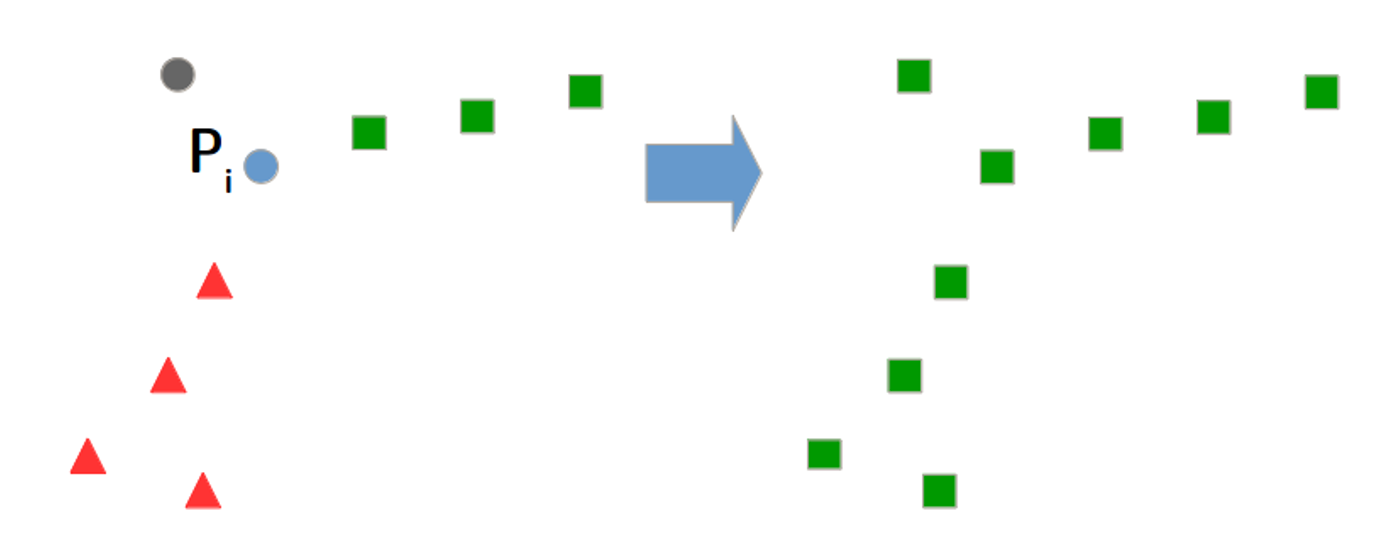
\includegraphics[width=0.8\textwidth]{resource/figures/condition3.png}
            \\ \tiny A joint point of multiple clusters. (Merge clusters)
           \column{0.5\textwidth}
            \centering
            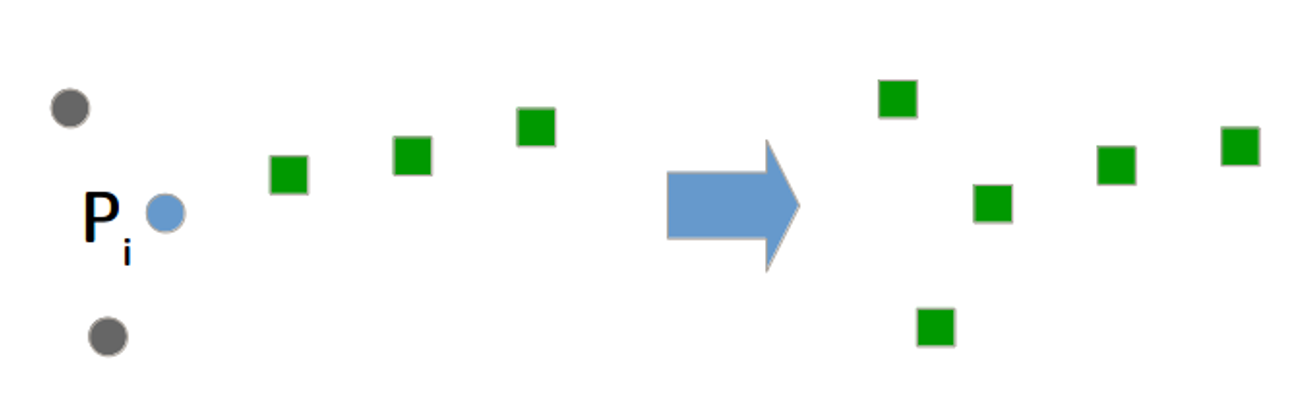
\includegraphics[width=0.8\textwidth]{resource/figures/condition4.png}
            \\ \tiny Extend an existing cluster.
    \end{columns}
\end{frame}

\begin{frame}
    \frametitle{Adapting the incremental DBSCAN to parallel processing}
    \begin{itemize}
        \item Simultaneously independent insertion of input points can lead to conflicts.
        \begin{itemize}
	        \item \small Each input point should know the other input data that is being processed in parallel.
	        \item \small Conflicts between the results of each parallel processor need to be solved before clusters are persisted.
        \end{itemize}
        \item It is hard to cluster data streams in a fully parallel manner, therefore master-slaves mode is employed.
        \item Adapt point-by-point insertion into tick-by-tick insertion.
        \begin{itemize}
            \item \tiny Data points from incoming data-streams are divided into separate ticks based on their arriving times
            \item \tiny Within each tick, data are processed and clustered in parallel.
            \item \tiny The results of each parallel processing step (within one tick) need to be merged before being persisted. To solve any/all conflicts in data consistency.
            \item \tiny At the end of each tick, the result must be persisted into the historical dataset (generate a new snapshot) before a new tick is started.
        \end{itemize}
    \end{itemize}
\end{frame}

\begin{frame}
    \frametitle{Tick-by-tick Growing of DBSCAN clusters}
    \begin{columns}
        \column{0.65\textwidth}
                \begin{columns}
                    \column{0.5\textwidth}
                        \centering             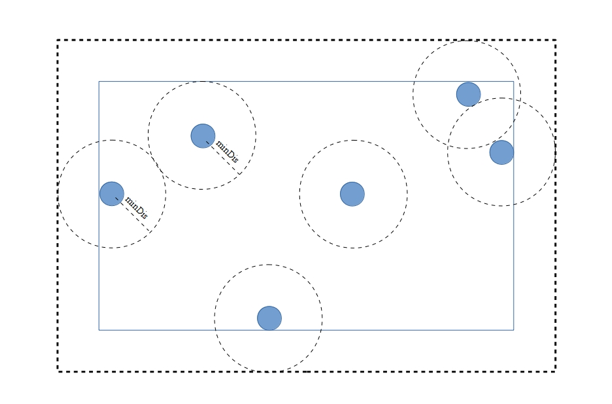
\includegraphics[width=0.8\textwidth]{resource/figures/boundingbox.png}
                    \column{0.5\textwidth}
                        \tiny Get the BBX for a group of inputs in a given tick.
                \end{columns}
            \centering
            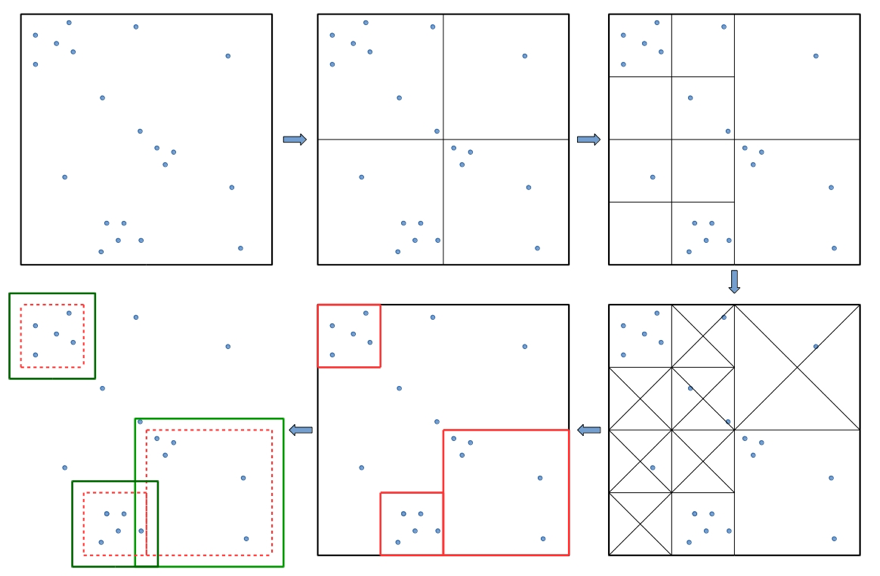
\includegraphics[width=\textwidth]{resource/figures/rt-dbscan.png}
        \column{0.35\textwidth}
        \small Fast Clustering (FC) partitioning
        \begin{itemize}
            \item \tiny Iteratively divide data space into sub-cells until a threshold is reached.
            \begin{itemize}
                \item \tiny Number of points within the cell is less than $maxPts$ ($=6$ in the left figure)
                \item \tiny The minimum border of current cell is less than $2\epsilon$
            \end{itemize}
            \item \tiny Drop the cells where the number of contained points is less than $minPts$ (3 in the figure) or there is no new input inside.
            \item \tiny Extend each quad-cell by $1-\epsilon$ distance on each border.
        \end{itemize}
    \end{columns}
\end{frame}

\begin{frame}
    \frametitle{Tick-by-tick Growing of DBSCAN clusters (2)}
    \begin{itemize}
	    \item Incremental DBSCANs are conducted in parallel for each cell.
	    \item A merging phase is executed at the end of each tick processing (before generating the result of each checkpoint)
	    \begin{itemize}
	        \item \small Solve conflicts between partitions/cells.
            \item \small Add ‘dropped’ new input (marked as noise during FC partition) into final result set.
            \item \small Identify unloaded data which belong to to-be-merged clusters.
	    \end{itemize}
    \end{itemize}
    \begin{figure}
        \centering
        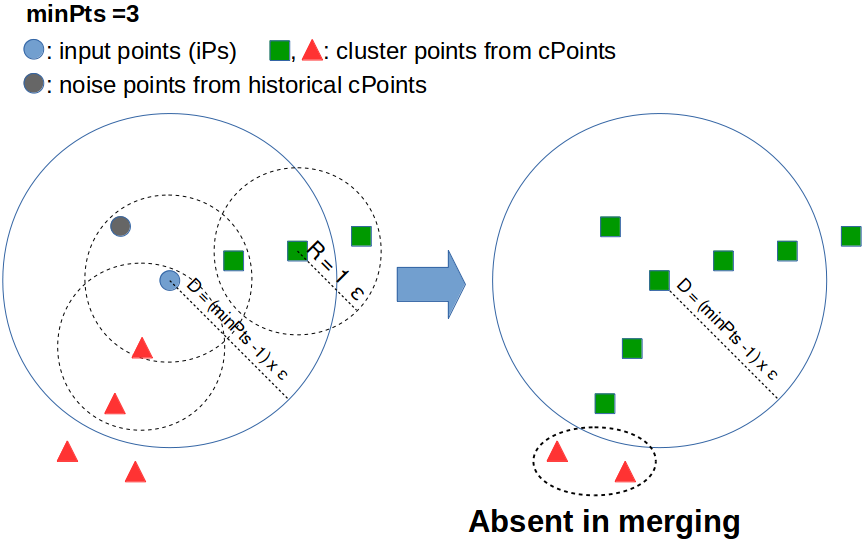
\includegraphics[width=0.46\textwidth]{resource/figures/merging-clusters.png}
    \end{figure}
\end{frame}

\begin{frame}
    \frametitle{RT-DBSCAN and its Implementation on SMASH/Spark}
    \begin{columns}
        \column{0.55\textwidth}
            \begin{itemize}
                \item \tiny Utilize Spark-Streaming which naturally support mirco-batch streaming processing.
                \item \tiny GeoMesa/Accumulo cluster offers efficient indexing strategy for querying nearby cluster knowledge over large-scale of Geographic data.
                \item \tiny Kafka is used as the streaming source for feeding new data.
            \end{itemize}
            \begin{figure}
                \centering
                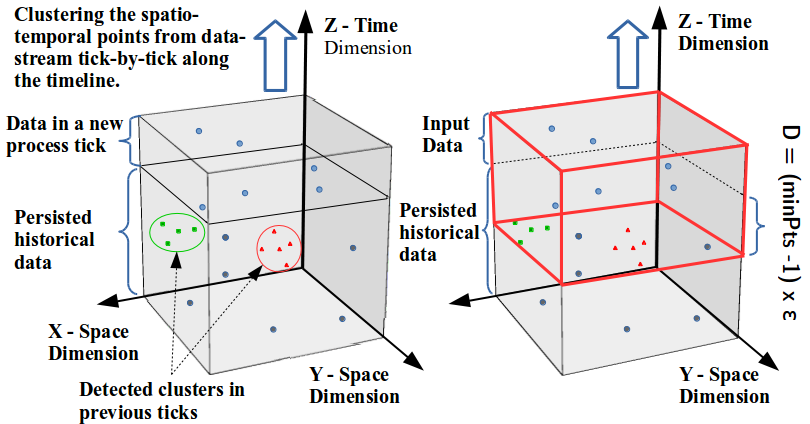
\includegraphics[width=\linewidth]{resource/figures/nearby-3d.png}
                \caption{\small An example of clustering the spatio-temporal data in a time tick}
            \end{figure}
        \column{0.45\textwidth}
        \begin{figure}
            \centering
            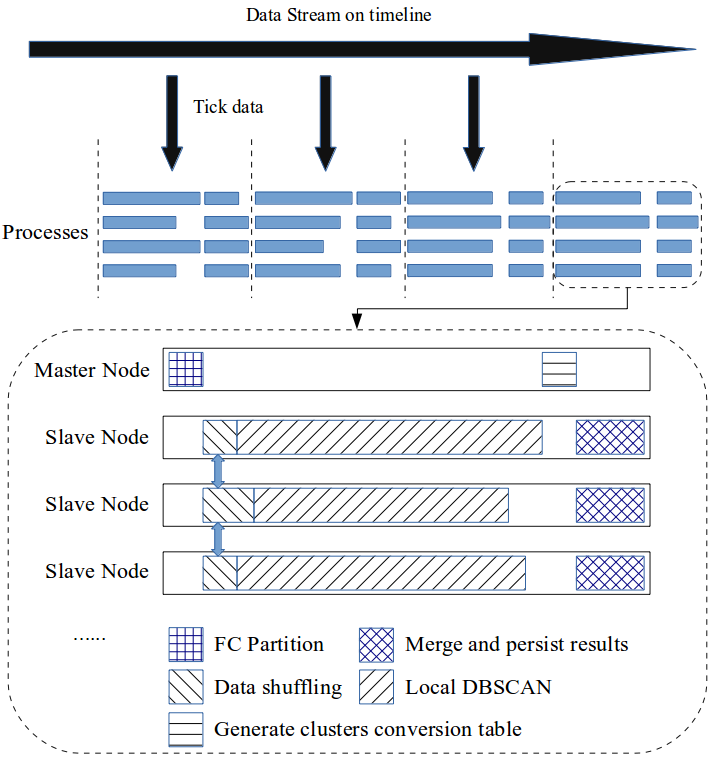
\includegraphics[width=\linewidth]{resource/figures/RT-DBSCAN_Spark.png}
            \caption{\small RT-DBSCAN processing using Spark-Streaming}
        \end{figure}
    \end{columns}
\end{frame}

\begin{frame}
    \frametitle{RT-DBSCAN Benchmarking}
    \begin{itemize} \small
	    \item  In a case-study benchmark, RT-DBSCAN is able to tackle data stream at over 10,000 social media data per second.
	    \item  The actual performance varies by the choices of parameter settings and the hardware performance.
	    \item The system is considered stable when: \\ {\it Batch Interval Time} $>$  {\it Batch Processing Time}
    \end{itemize}
    \begin{figure}
        \centering
        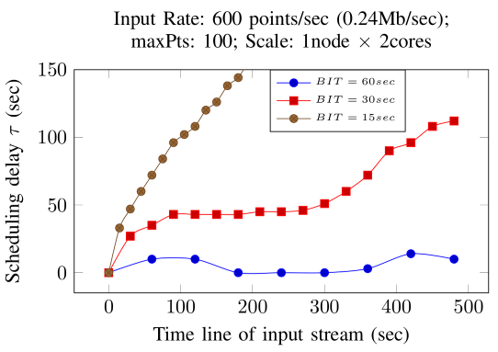
\includegraphics[width=0.44\linewidth]{resource/figures/rt-dbscan_banchmark.png}
        \vspace{-0.5cm}
        \caption{\small Performance Benchmarking using Different BIT Values}
    \end{figure}
\end{frame}

%==============================
\section{Case-studies}
%==============================

%----------------------------
\subsection{Data Description}
\begin{frame}
    \frametitle{}
    \begin{itemize}
	    \item SCATS Traffic Volume Data
	    \begin{itemize} \small
	        \item An official public urban traffic data source provided by the Australian government agency.
	        \item SCATS system utilizes a wide coverage sensor network on the major roads to monitor the traffic status and control the traffic flow by smart traffic lights.
	        \item SCATS Traffic Volume Data collected throughout 2017 in Victoria are used in the case-studies.
	    \end{itemize}
	    \item Social Media Data
	        \begin{itemize} \small
	            \item Collected from the public API of social media provider (e.g, Twitter, Instagram)
	            \item Social Media data created from 01/06/2017 to 31/12/2017 in Melbourne area used in the case-studies
	            \item After pre-processing, there are 132,927 GPS tag attached social media entities (tweets/posts) used for the case-studies.
	        \end{itemize}
    \end{itemize}
\end{frame}

%----------------------------
\subsection{Observations on the Social Media Clusters via SMASH}
\begin{frame}
    \frametitle{}
    \begin{figure}		  
	    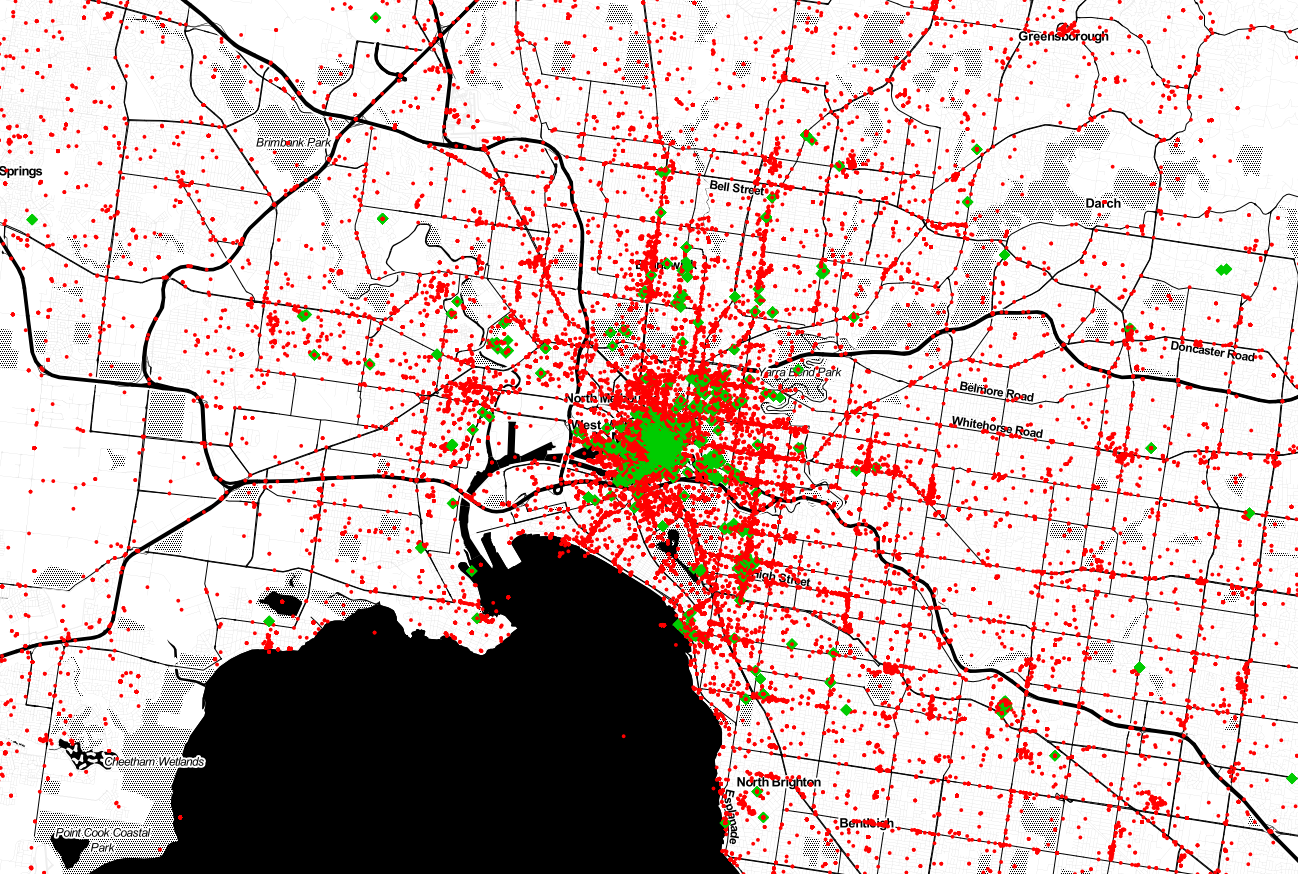
\includegraphics[width=0.95\columnwidth]{resource/figures/clustered_social_media_overview}
	    \centering
	    \vspace{-0.3cm}
	    \caption{\small An Overview the Processed Social Media Data}
    \end{figure}
\end{frame}

\begin{frame}
    \frametitle{}
    \begin{figure}		  
	    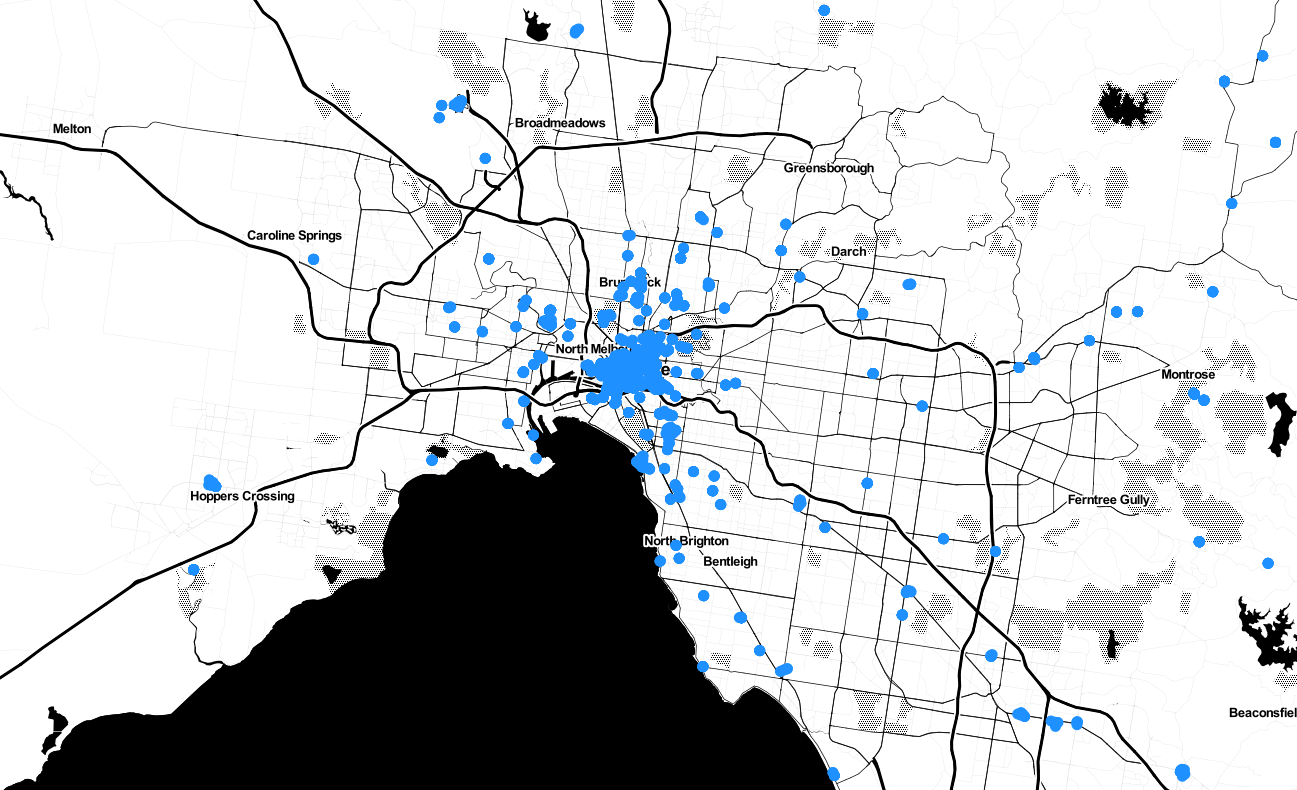
\includegraphics[width=0.95\columnwidth]{resource/figures/socialmedia_clusters.png}
	    \centering
	    \vspace{-0.3cm}
	    \caption{\small An Overview of the identified Social Media Data Clusters}
    \end{figure}
\end{frame}

\begin{frame}
    \frametitle{}
    \begin{figure}		  
    	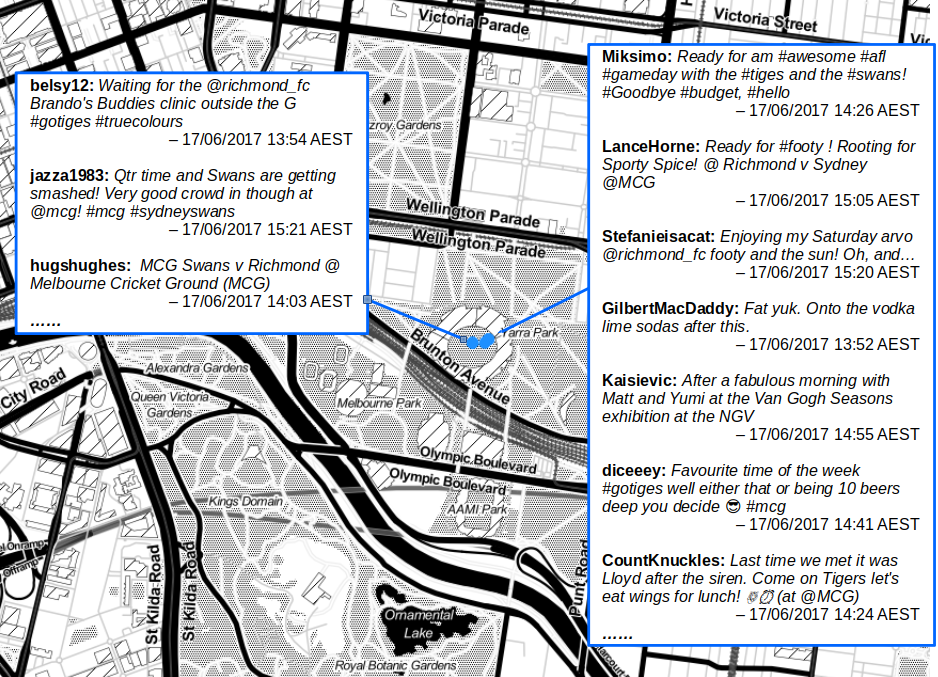
\includegraphics[width=0.88\columnwidth]{resource/figures/cluster_1e.png}
    	\centering
    	\vspace{-0.2cm}
    	\caption{\tiny A given detected social media cluster in/near Melbourne Cricket Ground on 17/06/2017 at around 2pm (local time)}
    \end{figure}
\end{frame}

\begin{frame}
    \frametitle{}
    \begin{figure}		  
    	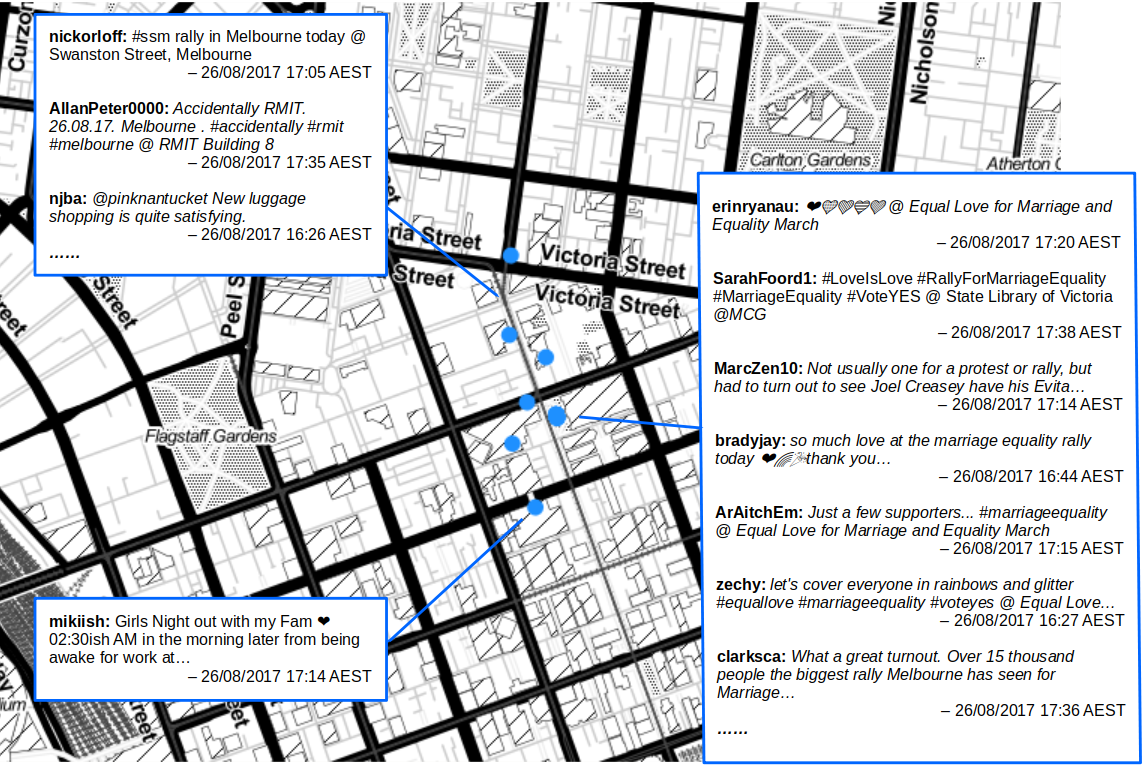
\includegraphics[width=0.95\columnwidth]{resource/figures/cluster_2e.png}
    	\centering
    	\vspace{-0.2cm}
    	\caption{\tiny A given detected social media cluster near the Victoria State Library on 26/08/2017 at around 5pm (local time).}
    \end{figure}
\end{frame}

%----------------------------
\subsection{Identifying Abnormal Traffic Volumes and Social Media Data}
\begin{frame}
    \frametitle{}
    This observation gives rise to a key question: can we find certain correlations between social media clusters such as abnormal spatio-temporal distributions and irregular patterns of human mobility such as urbantraffic abnormalities?
    \begin{itemize} \small
        \item How to define abnormal patterns of social media data and  abnormal patterns of urban traffic volumes?
        \item For a detected urban traffic abnormality, can we find any corresponding (nearby) social media abnormalities?
        \item For a detected social media abnormality, can we find any corresponding (nearby) urban traffic abnormalities?
    \end{itemize}
\end{frame}

\begin{frame}
    \frametitle{Generate baseline for Abnormality Detection}
    \begin{itemize}
	    \item Generate a baseline for traffic volumes at eachsensor spot on each day of the week and at each hour of the day.
	    \begin{itemize} \small
	        \item Standard deviations ($\sigma$) are calculated for the average traffic volumes.
	        \item Volumes which do not fit within the range $Avg\pm2\sigma$ are identified as irregular traffic patterns.
	    \end{itemize}
	    \item Similarly, a baseline of social media data is generated based on their distance to the nearby SCATS sensors.
	    \begin{itemize} \small
	        \item By aggregating (clustering) nearby social media data within 1 km distance to the SCATS sensor
	        \item When SCATS data are not present, it is reasonable to use the clustering information of social media alone for identifying abnormalities.
	    \end{itemize}
    \end{itemize}
\end{frame}

\begin{frame}
    \frametitle{}
    \begin{figure}
    	\centering
    	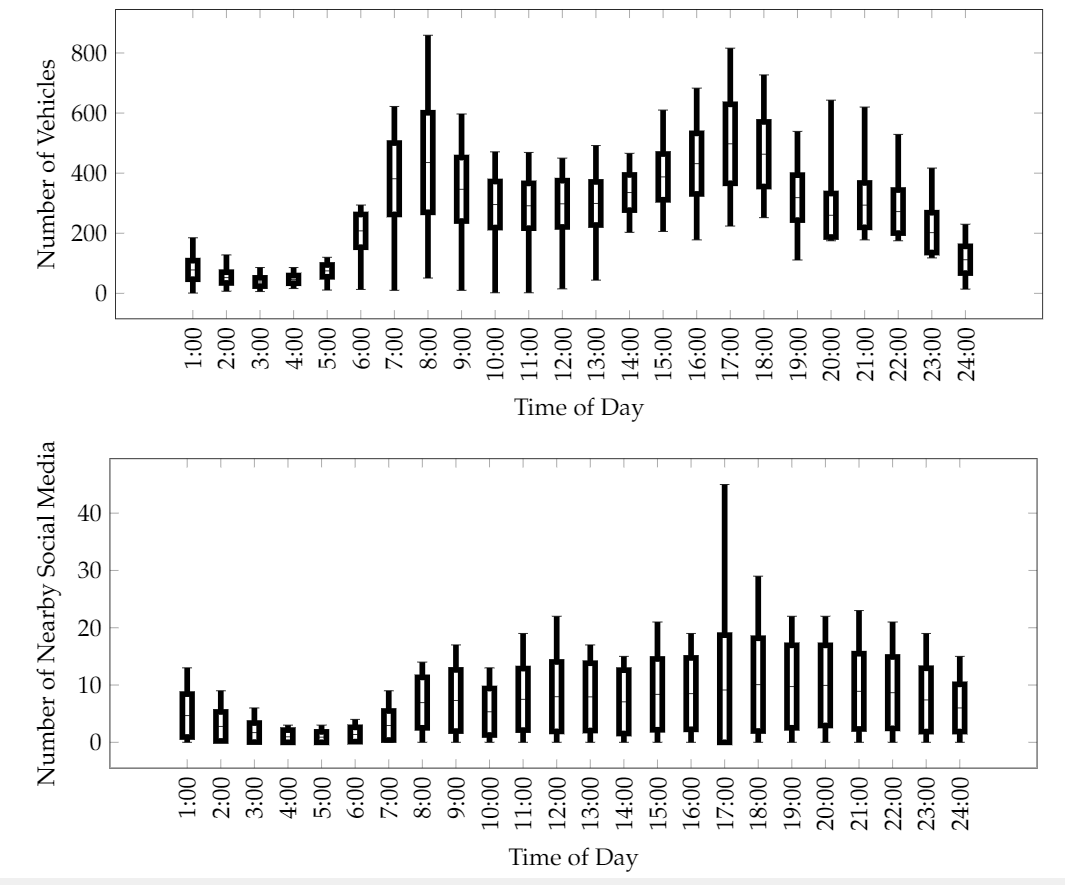
\includegraphics[width=0.7\columnwidth]{resource/figures/box_plot.png}
    	\caption{Box plot of traffic volume and nearby (within 1km distance) social media volume on Mondays at Princes Bridge, Melbourne}
    \end{figure}
\end{frame}


%----------------------------
\subsection{Traffic Data-driven Abnormality Analysis}
\begin{frame}
    \frametitle{Traffic Data-driven Abnormality Analysis}
    Procedure:
    \begin{itemize}
	    \item Baseline generation
	    \item Traffic volume abnormality detection
	    \item Looking at nearby social media data (for abnormalities)
	    \item Generating report and calculate Odds/Risk Ratio \cite{lipsitz1991generalized}
	    \begin{itemize} \small 
	        \item {\it abnormal-traffic with abnormal-social-media} (TT)
	        \item {\it abnormal-traffic with normal-social-media} (TF)
	        \item {\it normal-traffic with abnormal-social-media} (FT)
	        \item {\it normal-traffic with normal-social-media} (FF)
	    \end{itemize}
    \end{itemize}
\end{frame}

\begin{frame}
    \frametitle{Odds Ratio and Risk Ratio}
    \small In statistics, the odds ratio (OR) and risk ratio \cite{cornfield1951method,mosteller1968association} are predominant ways to quantify how strongly the presence or absence of property $A$ is associated with the presence or absence of property $B$ in a given population.
    \begin{itemize} \tiny
        \item If the value of the OR is above $1$, then it can be inferred that the presence of property $A$ (traffic volume abnormality) can be considered as `associated' with the presence of property $B$ (abnormality in the surrounding social media)
        \item The higher the value of OR, the stronger the association.
    \end{itemize}
    \begin{equation}
        \tiny
        \begin{split}
        OR &= \frac{\text{Odds of traffic abnormality in abnormal socmed group}}{\text{Odds of traffic abnormality in normal socmed group}\hfill} \\
           &= \frac{N_{TT} / N_{FT}}{N_{TF} / N_{FF}}
        \end{split}
        \label{eq:od}
    \end{equation}
    \begin{equation}
        \tiny
        \begin{split}
        RR &=\frac{\text{Risk of traffic abnormality in abnormal socmed group}}{\text{Risk of traffic abnormality in normal socmed group}\hfill} \\
           &= \frac{N_{TT} / (N_{TT} + N_{FT})}{N_{TF} / (N_{TF} + N_{FF})}
        \end{split}
        \label{eq:rr}
    \end{equation}
\end{frame}

\begin{frame}
    \frametitle{Results}
    \begin{figure}
        \centering
        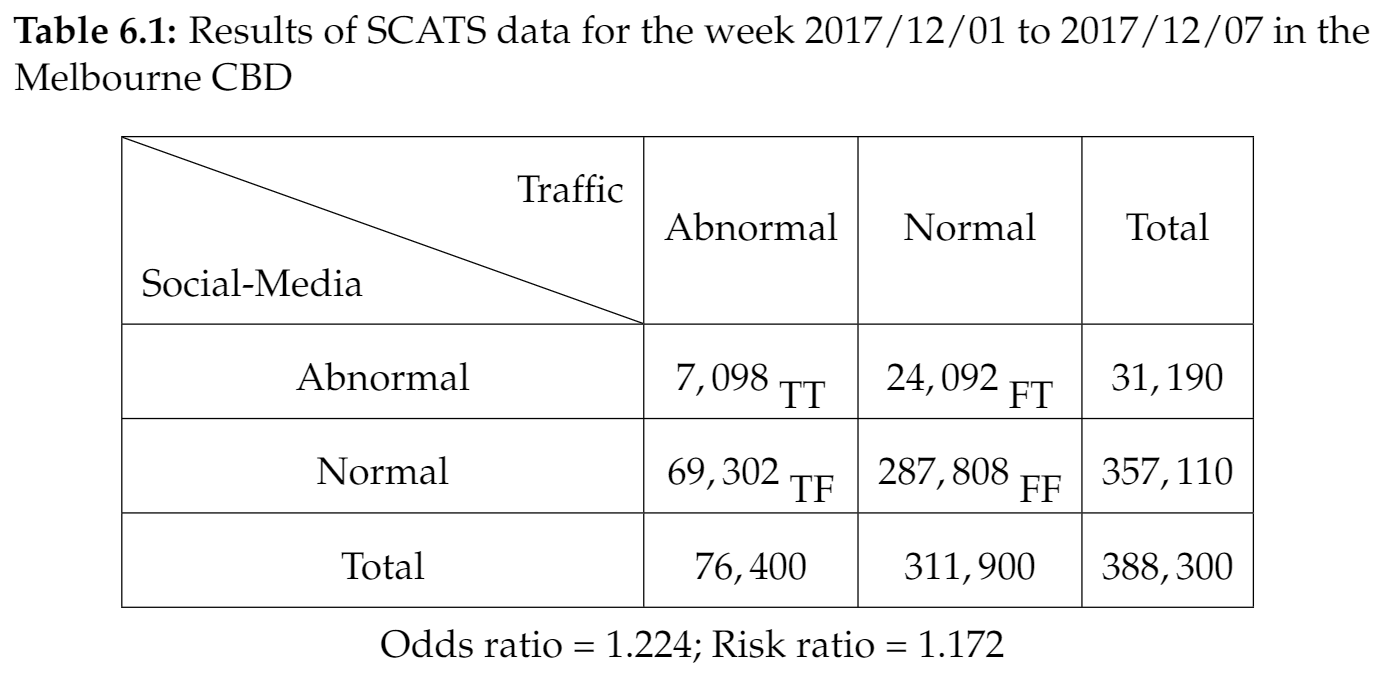
\includegraphics[width=0.7\columnwidth]{resource/figures/odds_ratio.png}
    \end{figure}
    \vspace{-0.2cm}
    \begin{itemize} \tiny
        \item The corresponding odds ratio is $1.224$ which is greater than $1$. This means that the presence of traffic volume abnormalities has a degree of correlation to the presence of nearby social-media distribution abnormalities.
        \item The risk ratio is 1.172 which implies that there is a higher risk in having traffic volume abnormalities when the distribution of nearby social-media is abnormal. This suggests that the abnormalities of social media distribution may have positive effects in predicting traffic abnormalities.
    \end{itemize}
\end{frame}

%----------------------------
\subsection{Social Media Data-driven Abnormality Analysis}
\begin{frame}
    \frametitle{}
	 For each detected social-media cluster, we checked its surrounding SCATS records for abnormal traffic flow volumes. 
	 \begin{itemize} \small
	       \item A spatio-temporal bounding box is calculated for retrieving the surrounding SCATS data for each social-media cluster.
	       \begin{itemize} \tiny
	            \item The temporal range of this bounding box starts from the earliest timestamp to the last timestamp among the social-media cluster members.
	            \item The spatial area of this bounding box is a circular area with a calculated radius.
	        \end{itemize}
	        \item A traffic volume abnormality is detected based on its baseline
	 \end{itemize}
	 \vspace{-0.15cm}
	 \begin{figure}
    	\centering
        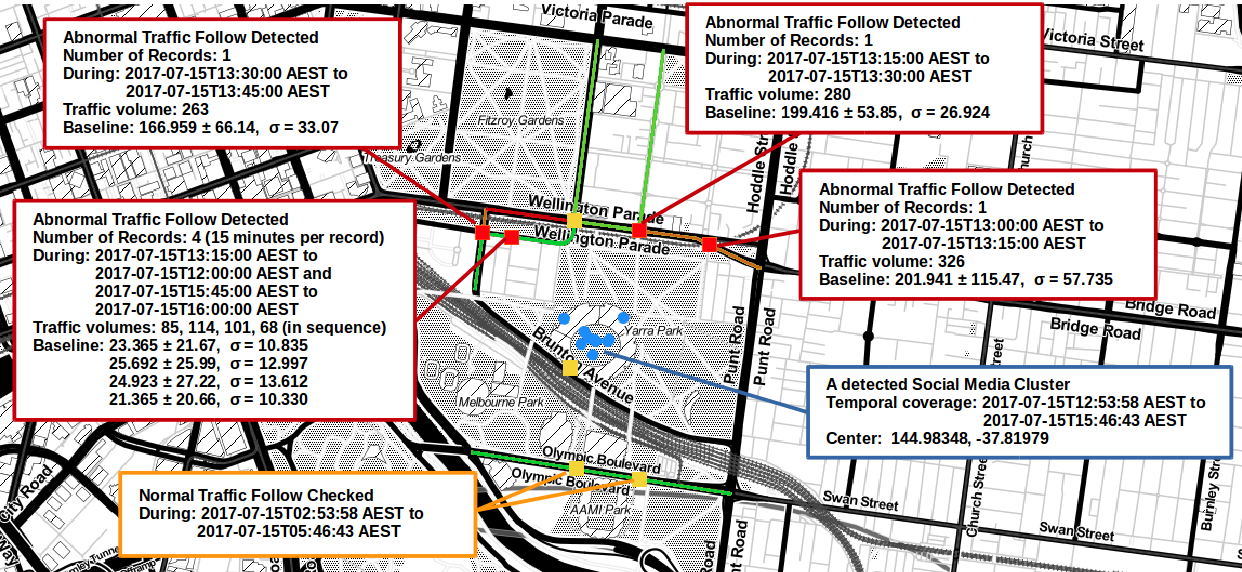
\includegraphics[width=.9\textwidth]{resource/figures/casestudy2_exp.png}
    \end{figure}
\end{frame}

\begin{frame}
    \frametitle{}
    \begin{columns}
        \column{0.5\columnwidth}
            \begin{figure}
            \centering
            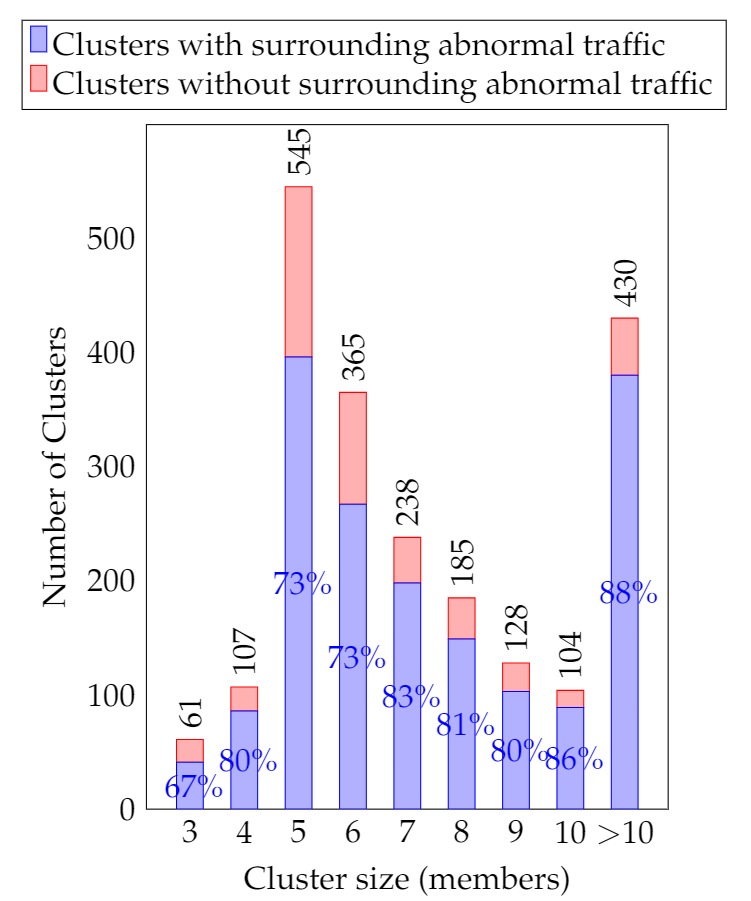
\includegraphics[width=\columnwidth]{resource/figures/caseStudy2_barChart.png}
            \vspace{-0.2cm}
        	\caption{\tiny Surrounding Traffic Abnormality Detection with Different Sizes of Social Media Clusters}
            \end{figure}
        \column{0.5\columnwidth}
            \begin{itemize} \small
                \item From the 2,261 detected clusters, we identify that most of them have 5 or 6 members (tweets/posts)
                \item Clusters with more members have a higher probability to have abnormal traffic volumes in their surrounding area. 
                \item The density of social media clusters can be used as a factor in calculating the confidence of traffic abnormality prediction when a social media cluster is identified in real-time.
            \end{itemize}
    \end{columns}
\end{frame}


%==============================
\section{Conclusions}
%==============================
\begin{frame}
    \frametitle{Conclusions}
    \begin{itemize} \small
	    \item A Cloud-based architecture --- SMASH is presented for conducting (real-time) Urban traffic analytics.
	    \item Proposed an equation for measuring spatio-temporal distance and demonstrated a method for harvesting social media data along the streets.
	    \item Proposed a real-time density-based clustering algorithm for processing Big Data stream on Cloud.
	    \begin{itemize}
	        \item It can be adapted to many other data fields as long as a customized measurement of distance/density is presented
	    \end{itemize}
	    \item We explored the spatio-temporal correlation between the abnormalities of Social Media Data and the official Urban Traffic Volume data. 
	    \begin{itemize}
	        \item Based on the statistic results, we think the spatio-temporal clusters of social-media data can be used as a proxy for traffic analytics.  
	    \end{itemize}
    \end{itemize}
\end{frame}

\begin{frame}
    \frametitle{Main Publications}
    \begin{itemize} \tiny
	    \item Y. Gong, L. Morandini, and R.O. Sinnott, The Design and Benchmarking of a Cloud-based Platform for Processing and Visualization of Traffic Data, in \emph{proceedings of the 4th IEEE International Conference on Big Data and Smart Computing}, Jeju Island, Korea, February 2017.
	    \item Y. Gong, F. Deng, and R.O. Sinnott, Identification of (near) Real-time Traffic Congestion in the Cities of Australia through Twitter, Understanding the City with Urban Informatics, in \emph{Proceedings of the 24th ACM International Conference on Information and Knowledge Management (CIKM)}, Melbourne, Australia, October 2015.
	    \item Y. Gong, P. Rimba, and R.O. Sinnott, RT-DBSCAN: Real-time Parallel Clustering of Spatio-Temporal Data using Spark-Streaming, in \emph{Proceedings of the International Conference on Computational Science (ICCS)}, Wuxi, China, June 2018.
	    \item Y. Gong, P. Rimba, and R.O. Sinnott, A Big Data Architecture for Near Real-time Traffic Analytics, in \emph{Proceedings of the 10th IEEE/ACM International Conference on Utility and Cloud Computing (UCC)}, Texas, USA, December 2017.
        \item Y. Gong, R.O. Sinnott, S. Chen, and P. Rimba, Urban Traffic Analysis using Social Media Data on the Cloud, in \emph{the 5th IEEE/ACM International Workshop on Smart City Clouds: Technologies, Systems and Applications}, Zurich, Switzerland, December 2018.
    \end{itemize}
\end{frame}

\begin{frame}[plain]
    \tiny
    \frametitle{References}
    \bibliographystyle{abbrv}
    \bibliography{resource/ref.bib}
\end{frame}

% \begin{frame}[plain]
%     \begin{center}
%         \Huge Thank you for the attention!
%         \vfill
%         \Large Your Name
%     \end{center}
% \end{frame}

\end{document}